\documentclass[1p]{elsarticle_modified}
%\bibliographystyle{elsarticle-num}

%\usepackage[colorlinks]{hyperref}
%\usepackage{abbrmath_seonhwa} %\Abb, \Ascr, \Acal ,\Abf, \Afrak
\usepackage{amsfonts}
\usepackage{amssymb}
\usepackage{amsmath}
\usepackage{amsthm}
\usepackage{scalefnt}
\usepackage{amsbsy}
\usepackage{kotex}
\usepackage{caption}
\usepackage{subfig}
\usepackage{color}
\usepackage{graphicx}
\usepackage{xcolor} %% white, black, red, green, blue, cyan, magenta, yellow
\usepackage{float}
\usepackage{setspace}
\usepackage{hyperref}

\usepackage{tikz}
\usetikzlibrary{arrows}

\usepackage{multirow}
\usepackage{array} % fixed length table
\usepackage{hhline}

%%%%%%%%%%%%%%%%%%%%%
\makeatletter
\renewcommand*\env@matrix[1][\arraystretch]{%
	\edef\arraystretch{#1}%
	\hskip -\arraycolsep
	\let\@ifnextchar\new@ifnextchar
	\array{*\c@MaxMatrixCols c}}
\makeatother %https://tex.stackexchange.com/questions/14071/how-can-i-increase-the-line-spacing-in-a-matrix
%%%%%%%%%%%%%%%

\usepackage[normalem]{ulem}

\newcommand{\msout}[1]{\ifmmode\text{\sout{\ensuremath{#1}}}\else\sout{#1}\fi}
%SOURCE: \msout is \stkout macro in https://tex.stackexchange.com/questions/20609/strikeout-in-math-mode

\newcommand{\cancel}[1]{
	\ifmmode
	{\color{red}\msout{#1}}
	\else
	{\color{red}\sout{#1}}
	\fi
}

\newcommand{\add}[1]{
	{\color{blue}\uwave{#1}}
}

\newcommand{\replace}[2]{
	\ifmmode
	{\color{red}\msout{#1}}{\color{blue}\uwave{#2}}
	\else
	{\color{red}\sout{#1}}{\color{blue}\uwave{#2}}
	\fi
}

\newcommand{\Sol}{\mathcal{S}} %segment
\newcommand{\D}{D} %diagram
\newcommand{\A}{\mathcal{A}} %arc


%%%%%%%%%%%%%%%%%%%%%%%%%%%%%5 test

\def\sl{\operatorname{\textup{SL}}(2,\Cbb)}
\def\psl{\operatorname{\textup{PSL}}(2,\Cbb)}
\def\quan{\mkern 1mu \triangleright \mkern 1mu}

\theoremstyle{definition}
\newtheorem{thm}{Theorem}[section]
\newtheorem{prop}[thm]{Proposition}
\newtheorem{lem}[thm]{Lemma}
\newtheorem{ques}[thm]{Question}
\newtheorem{cor}[thm]{Corollary}
\newtheorem{defn}[thm]{Definition}
\newtheorem{exam}[thm]{Example}
\newtheorem{rmk}[thm]{Remark}
\newtheorem{alg}[thm]{Algorithm}

\newcommand{\I}{\sqrt{-1}}
\begin{document}

%\begin{frontmatter}
%
%\title{Boundary parabolic representations of knots up to 8 crossings}
%
%%% Group authors per affiliation:
%\author{Yunhi Cho} 
%\address{Department of Mathematics, University of Seoul, Seoul, Korea}
%\ead{yhcho@uos.ac.kr}
%
%
%\author{Seonhwa Kim} %\fnref{s_kim}}
%\address{Center for Geometry and Physics, Institute for Basic Science, Pohang, 37673, Korea}
%\ead{ryeona17@ibs.re.kr}
%
%\author{Hyuk Kim}
%\address{Department of Mathematical Sciences, Seoul National University, Seoul 08826, Korea}
%\ead{hyukkim@snu.ac.kr}
%
%\author{Seokbeom Yoon}
%\address{Department of Mathematical Sciences, Seoul National University, Seoul, 08826,  Korea}
%\ead{sbyoon15@snu.ac.kr}
%
%\begin{abstract}
%We find all boundary parabolic representation of knots up to 8 crossings.
%
%\end{abstract}
%\begin{keyword}
%    \MSC[2010] 57M25 
%\end{keyword}
%
%\end{frontmatter}

%\linenumbers
%\tableofcontents
%
\newcommand\colored[1]{\textcolor{white}{\rule[-0.35ex]{0.8em}{1.4ex}}\kern-0.8em\color{red} #1}%
%\newcommand\colored[1]{\textcolor{white}{ #1}\kern-2.17ex	\textcolor{white}{ #1}\kern-1.81ex	\textcolor{white}{ #1}\kern-2.15ex\color{red}#1	}

{\Large $\underline{11a_{338}~(K11a_{338})}$}

\setlength{\tabcolsep}{10pt}
\renewcommand{\arraystretch}{1.6}
\vspace{1cm}\begin{tabular}{m{100pt}>{\centering\arraybackslash}m{274pt}}
\multirow{5}{120pt}{
	\centering
	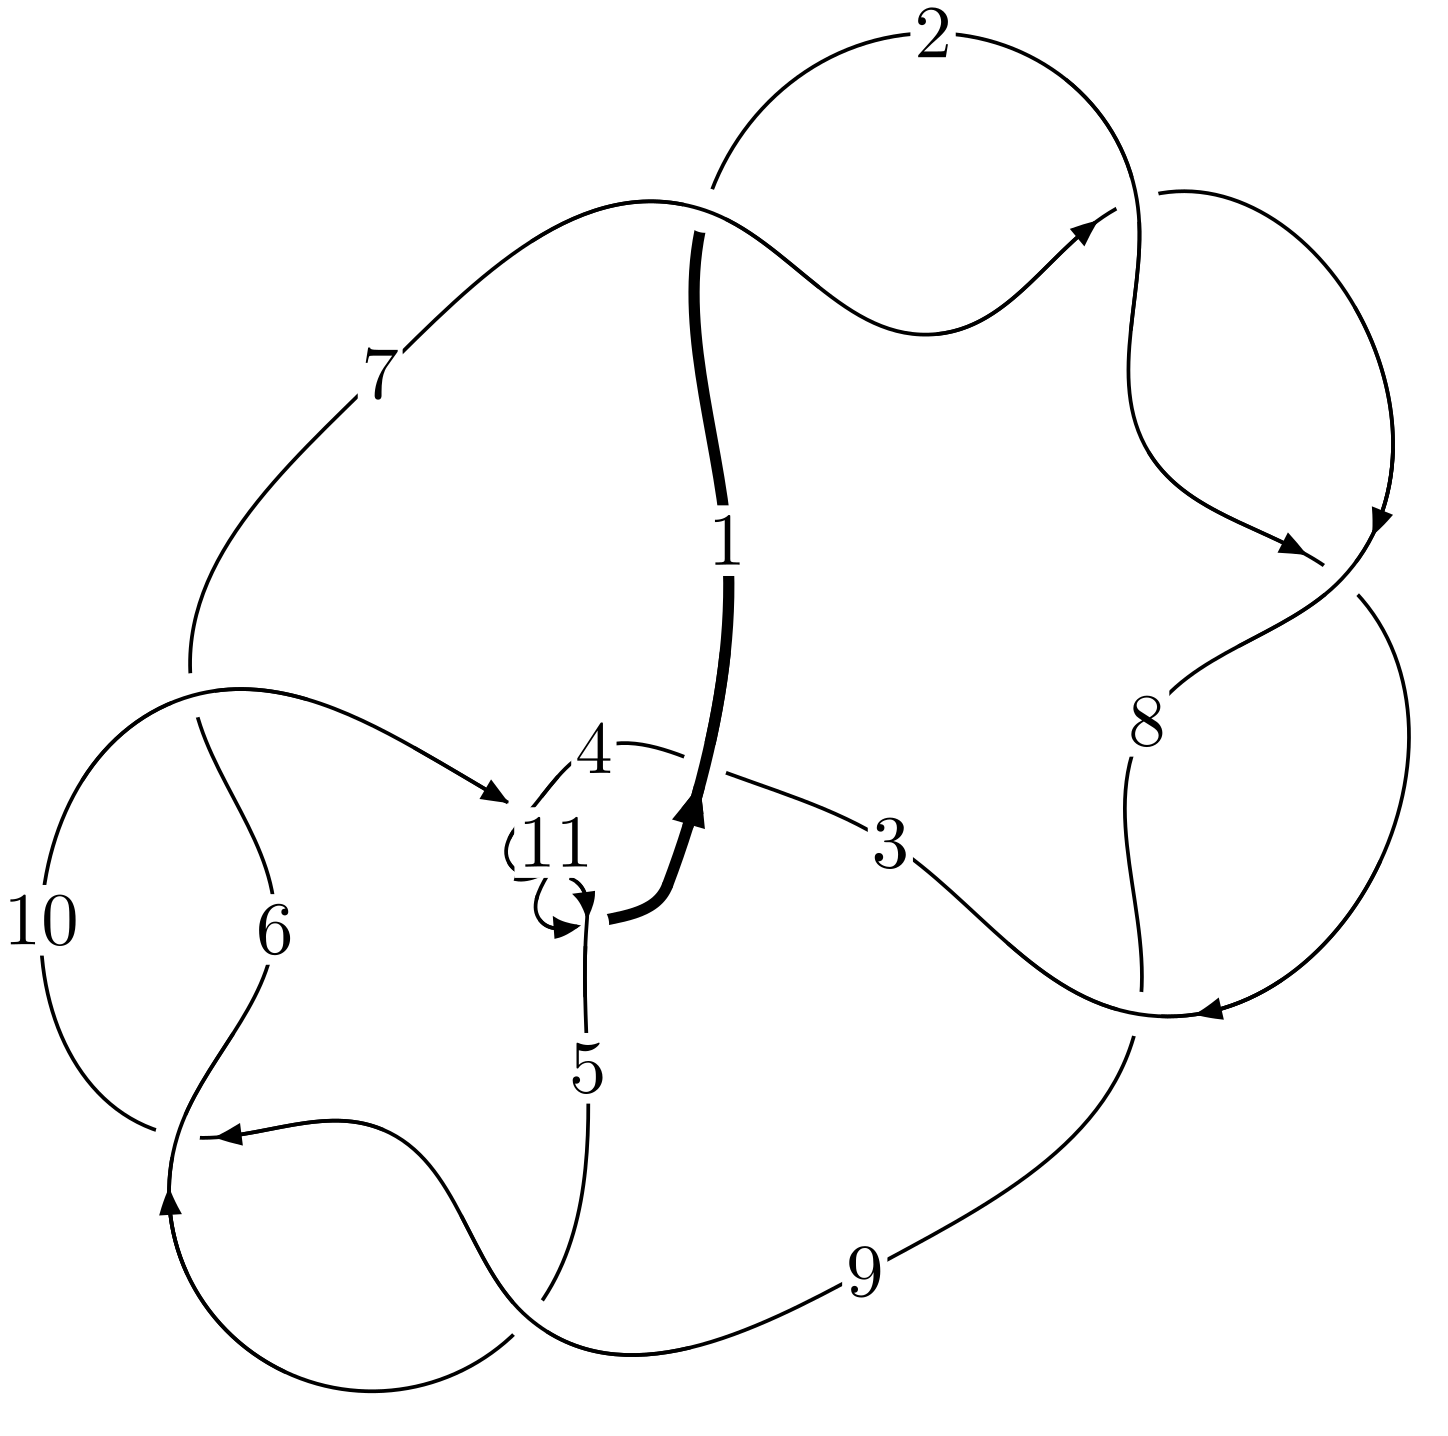
\includegraphics[width=112pt]{../../../GIT/diagram.site/Diagrams/png/587_11a_338.png}\\
\ \ \ A knot diagram\footnotemark}&
\allowdisplaybreaks
\textbf{Linearized knot diagam} \\
\cline{2-2}
 &
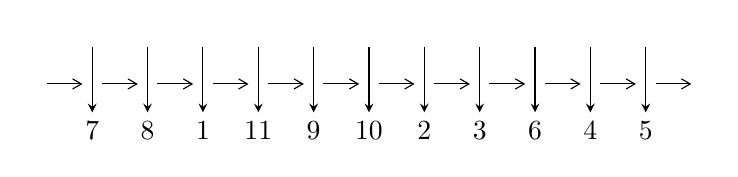
\begin{tikzpicture}[x=20pt, y=17pt]
	% nodes
	\node (C0) at (0, 0) {};
	\node (C1) at (1, 0) {};
	\node (C1U) at (1, +1) {};
	\node (C1D) at (1, -1) {7};

	\node (C2) at (2, 0) {};
	\node (C2U) at (2, +1) {};
	\node (C2D) at (2, -1) {8};

	\node (C3) at (3, 0) {};
	\node (C3U) at (3, +1) {};
	\node (C3D) at (3, -1) {1};

	\node (C4) at (4, 0) {};
	\node (C4U) at (4, +1) {};
	\node (C4D) at (4, -1) {11};

	\node (C5) at (5, 0) {};
	\node (C5U) at (5, +1) {};
	\node (C5D) at (5, -1) {9};

	\node (C6) at (6, 0) {};
	\node (C6U) at (6, +1) {};
	\node (C6D) at (6, -1) {10};

	\node (C7) at (7, 0) {};
	\node (C7U) at (7, +1) {};
	\node (C7D) at (7, -1) {2};

	\node (C8) at (8, 0) {};
	\node (C8U) at (8, +1) {};
	\node (C8D) at (8, -1) {3};

	\node (C9) at (9, 0) {};
	\node (C9U) at (9, +1) {};
	\node (C9D) at (9, -1) {6};

	\node (C10) at (10, 0) {};
	\node (C10U) at (10, +1) {};
	\node (C10D) at (10, -1) {4};

	\node (C11) at (11, 0) {};
	\node (C11U) at (11, +1) {};
	\node (C11D) at (11, -1) {5};
	\node (C12) at (12, 0) {};

	% arrows
	\draw[->,>={angle 60}]
	(C0) edge (C1) (C1) edge (C2) (C2) edge (C3) (C3) edge (C4) (C4) edge (C5) (C5) edge (C6) (C6) edge (C7) (C7) edge (C8) (C8) edge (C9) (C9) edge (C10) (C10) edge (C11) (C11) edge (C12) ;	\draw[->,>=stealth]
	(C1U) edge (C1D) (C2U) edge (C2D) (C3U) edge (C3D) (C4U) edge (C4D) (C5U) edge (C5D) (C6U) edge (C6D) (C7U) edge (C7D) (C8U) edge (C8D) (C9U) edge (C9D) (C10U) edge (C10D) (C11U) edge (C11D) ;
	\end{tikzpicture} \\
\hhline{~~} \\& 
\textbf{Solving Sequence} \\ \cline{2-2} 
 &
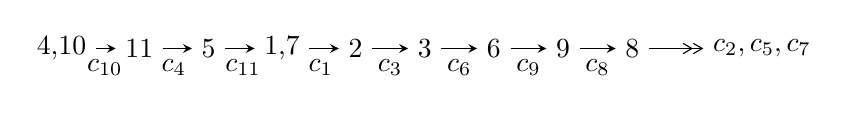
\begin{tikzpicture}[x=25pt, y=7pt]
	% node
	\node (A0) at (-1/8, 0) {4,10};
	\node (A1) at (1, 0) {11};
	\node (A2) at (2, 0) {5};
	\node (A3) at (49/16, 0) {1,7};
	\node (A4) at (33/8, 0) {2};
	\node (A5) at (41/8, 0) {3};
	\node (A6) at (49/8, 0) {6};
	\node (A7) at (57/8, 0) {9};
	\node (A8) at (65/8, 0) {8};
	\node (C1) at (1/2, -1) {$c_{10}$};
	\node (C2) at (3/2, -1) {$c_{4}$};
	\node (C3) at (5/2, -1) {$c_{11}$};
	\node (C4) at (29/8, -1) {$c_{1}$};
	\node (C5) at (37/8, -1) {$c_{3}$};
	\node (C6) at (45/8, -1) {$c_{6}$};
	\node (C7) at (53/8, -1) {$c_{9}$};
	\node (C8) at (61/8, -1) {$c_{8}$};
	\node (A9) at (10, 0) {$c_{2},c_{5},c_{7}$};

	% edge
	\draw[->,>=stealth]	
	(A0) edge (A1) (A1) edge (A2) (A2) edge (A3) (A3) edge (A4) (A4) edge (A5) (A5) edge (A6) (A6) edge (A7) (A7) edge (A8) ;
	\draw[->>,>={angle 60}]	
	(A8) edge (A9);
\end{tikzpicture} \\ 

\end{tabular} \\

\footnotetext{
The image of knot diagram is generated by the software ``\textbf{Draw programme}" developed by Andrew Bartholomew(\url{http://www.layer8.co.uk/maths/draw/index.htm\#Running-draw}), where we modified some parts for our purpose(\url{https://github.com/CATsTAILs/LinksPainter}).
}\phantom \\ \newline 
\centering \textbf{Ideals for irreducible components\footnotemark of $X_{\text{par}}$} 
 
\begin{align*}
I^u_{1}&=\langle 
b- u,\;u^{14}+u^{13}-7 u^{12}-6 u^{11}+18 u^{10}+11 u^9-18 u^8- u^7+u^6-12 u^5+5 u^4+2 u^2+2 a+7 u,\\
\phantom{I^u_{1}}&\phantom{= \langle  }u^{15}+u^{14}-8 u^{13}-7 u^{12}+25 u^{11}+17 u^{10}-36 u^9-12 u^8+19 u^7-11 u^6+4 u^5+12 u^4-3 u^3+5 u^2-2 u-1\rangle \\
I^u_{2}&=\langle 
4397 u^{21}+2494 u^{20}+\cdots+8689 b-8433,\;-13086 u^{21}-11183 u^{20}+\cdots+8689 a+43189,\\
\phantom{I^u_{2}}&\phantom{= \langle  }u^{22}+u^{21}+\cdots-4 u+1\rangle \\
I^u_{3}&=\langle 
b-1,\;a^2-2,\;u+1\rangle \\
I^u_{4}&=\langle 
b+1,\;a,\;u-1\rangle \\
\\
\end{align*}
\raggedright * 4 irreducible components of $\dim_{\mathbb{C}}=0$, with total 40 representations.\\
\footnotetext{All coefficients of polynomials are rational numbers. But the coefficients are sometimes approximated in decimal forms when there is not enough margin.}
\newpage
\renewcommand{\arraystretch}{1}
\centering \section*{I. $I^u_{1}= \langle b- u,\;u^{14}+u^{13}+\cdots+2 a+7 u,\;u^{15}+u^{14}+\cdots-2 u-1 \rangle$}
\flushleft \textbf{(i) Arc colorings}\\
\begin{tabular}{m{7pt} m{180pt} m{7pt} m{180pt} }
\flushright $a_{4}=$&$\begin{pmatrix}0\\u\end{pmatrix}$ \\
\flushright $a_{10}=$&$\begin{pmatrix}1\\0\end{pmatrix}$ \\
\flushright $a_{11}=$&$\begin{pmatrix}1\\u^2\end{pmatrix}$ \\
\flushright $a_{5}=$&$\begin{pmatrix}- u\\- u^3+u\end{pmatrix}$ \\
\flushright $a_{1}=$&$\begin{pmatrix}- u^2+1\\- u^4+2 u^2\end{pmatrix}$ \\
\flushright $a_{7}=$&$\begin{pmatrix}-\frac{1}{2} u^{14}-\frac{1}{2} u^{13}+\cdots- u^2-\frac{7}{2} u\\u\end{pmatrix}$ \\
\flushright $a_{2}=$&$\begin{pmatrix}-\frac{1}{2} u^{14}+4 u^{12}+\cdots-\frac{3}{2} u+\frac{1}{2}\\\frac{1}{2} u^{13}+\frac{1}{2} u^{12}+\cdots+u+\frac{1}{2}\end{pmatrix}$ \\
\flushright $a_{3}=$&$\begin{pmatrix}u^5-2 u^3+u\\u^7-3 u^5+2 u^3+u\end{pmatrix}$ \\
\flushright $a_{6}=$&$\begin{pmatrix}-\frac{1}{2} u^{14}-\frac{1}{2} u^{13}+\cdots- u^2-\frac{5}{2} u\\u\end{pmatrix}$ \\
\flushright $a_{9}=$&$\begin{pmatrix}\frac{1}{2} u^{13}+\frac{1}{2} u^{12}+\cdots+u+\frac{3}{2}\\- u^2\end{pmatrix}$ \\
\flushright $a_{8}=$&$\begin{pmatrix}\frac{1}{2} u^{13}+\frac{1}{2} u^{12}+\cdots+u+\frac{3}{2}\\-\frac{1}{2} u^{13}+\frac{1}{2} u^{12}+\cdots- u-\frac{1}{2}\end{pmatrix}$\\ \flushright $a_{8}=$&$\begin{pmatrix}\frac{1}{2} u^{13}+\frac{1}{2} u^{12}+\cdots+u+\frac{3}{2}\\-\frac{1}{2} u^{13}+\frac{1}{2} u^{12}+\cdots- u-\frac{1}{2}\end{pmatrix}$\\&\end{tabular}
\flushleft \textbf{(ii) Obstruction class $= -1$}\\~\\
\flushleft \textbf{(iii) Cusp Shapes $= u^{14}+u^{13}-9 u^{12}-6 u^{11}+32 u^{10}+9 u^9-56 u^8+11 u^7+45 u^6-38 u^5-3 u^4+20 u^3-16 u^2+7 u-16$}\\~\\
\newpage\renewcommand{\arraystretch}{1}
\flushleft \textbf{(iv) u-Polynomials at the component}\newline \\
\begin{tabular}{m{50pt}|m{274pt}}
Crossings & \hspace{64pt}u-Polynomials at each crossing \\
\hline $$\begin{aligned}c_{1},c_{2},c_{7}\\c_{8}\end{aligned}$$&$\begin{aligned}
&u^{15}+3 u^{14}+\cdots+2 u+2
\end{aligned}$\\
\hline $$\begin{aligned}c_{3}\end{aligned}$$&$\begin{aligned}
&u^{15}-3 u^{14}+\cdots+16 u+16
\end{aligned}$\\
\hline $$\begin{aligned}c_{4},c_{5},c_{6}\\c_{9},c_{10},c_{11}\end{aligned}$$&$\begin{aligned}
&u^{15}+u^{14}+\cdots-2 u-1
\end{aligned}$\\
\hline
\end{tabular}\\~\\
\newpage\renewcommand{\arraystretch}{1}
\flushleft \textbf{(v) Riley Polynomials at the component}\newline \\
\begin{tabular}{m{50pt}|m{274pt}}
Crossings & \hspace{64pt}Riley Polynomials at each crossing \\
\hline $$\begin{aligned}c_{1},c_{2},c_{7}\\c_{8}\end{aligned}$$&$\begin{aligned}
&y^{15}-17 y^{14}+\cdots+36 y-4
\end{aligned}$\\
\hline $$\begin{aligned}c_{3}\end{aligned}$$&$\begin{aligned}
&y^{15}- y^{14}+\cdots+5376 y-256
\end{aligned}$\\
\hline $$\begin{aligned}c_{4},c_{5},c_{6}\\c_{9},c_{10},c_{11}\end{aligned}$$&$\begin{aligned}
&y^{15}-17 y^{14}+\cdots+14 y-1
\end{aligned}$\\
\hline
\end{tabular}\\~\\
\newpage\flushleft \textbf{(vi) Complex Volumes and Cusp Shapes}
$$\begin{array}{c|c|c}  
\text{Solutions to }I^u_{1}& \I (\text{vol} + \sqrt{-1}CS) & \text{Cusp shape}\\
 \hline 
\begin{aligned}
u &= \phantom{-}0.279761 + 0.693754 I \\
a &= -0.39605 - 1.71486 I \\
b &= \phantom{-}0.279761 + 0.693754 I\end{aligned}
 & -5.13135 - 3.51735 I & -12.62019 + 4.61757 I \\ \hline\begin{aligned}
u &= \phantom{-}0.279761 - 0.693754 I \\
a &= -0.39605 + 1.71486 I \\
b &= \phantom{-}0.279761 - 0.693754 I\end{aligned}
 & -5.13135 + 3.51735 I & -12.62019 - 4.61757 I \\ \hline\begin{aligned}
u &= -0.103670 + 0.625168 I \\
a &= \phantom{-}0.16824 - 1.53722 I \\
b &= -0.103670 + 0.625168 I\end{aligned}
 & \phantom{-}1.57961 + 1.61537 I & -7.48885 - 5.36345 I \\ \hline\begin{aligned}
u &= -0.103670 - 0.625168 I \\
a &= \phantom{-}0.16824 + 1.53722 I \\
b &= -0.103670 - 0.625168 I\end{aligned}
 & \phantom{-}1.57961 - 1.61537 I & -7.48885 + 5.36345 I \\ \hline\begin{aligned}
u &= -1.395200 + 0.215840 I \\
a &= -0.96796 - 1.31763 I \\
b &= -1.395200 + 0.215840 I\end{aligned}
 & -6.90209 + 4.05844 I & -16.6421 - 2.1211 I \\ \hline\begin{aligned}
u &= -1.395200 - 0.215840 I \\
a &= -0.96796 + 1.31763 I \\
b &= -1.395200 - 0.215840 I\end{aligned}
 & -6.90209 - 4.05844 I & -16.6421 + 2.1211 I \\ \hline\begin{aligned}
u &= \phantom{-}1.409280 + 0.090877 I \\
a &= \phantom{-}1.33372 - 0.62354 I \\
b &= \phantom{-}1.409280 + 0.090877 I\end{aligned}
 & -11.36840 - 0.36520 I & -21.3793 - 0.0972 I \\ \hline\begin{aligned}
u &= \phantom{-}1.409280 - 0.090877 I \\
a &= \phantom{-}1.33372 + 0.62354 I \\
b &= \phantom{-}1.409280 - 0.090877 I\end{aligned}
 & -11.36840 + 0.36520 I & -21.3793 + 0.0972 I \\ \hline\begin{aligned}
u &= \phantom{-}0.549904\phantom{ +0.000000I} \\
a &= -2.12645\phantom{ +0.000000I} \\
b &= \phantom{-}0.549904\phantom{ +0.000000I}\end{aligned}
 & -6.65878\phantom{ +0.000000I} & -14.7970\phantom{ +0.000000I} \\ \hline\begin{aligned}
u &= \phantom{-}1.42511 + 0.29485 I \\
a &= \phantom{-}0.56952 - 1.44587 I \\
b &= \phantom{-}1.42511 + 0.29485 I\end{aligned}
 & -8.40818 - 8.56529 I & -18.2568 + 6.8115 I\\
 \hline 
 \end{array}$$\newpage$$\begin{array}{c|c|c}  
\text{Solutions to }I^u_{1}& \I (\text{vol} + \sqrt{-1}CS) & \text{Cusp shape}\\
 \hline 
\begin{aligned}
u &= \phantom{-}1.42511 - 0.29485 I \\
a &= \phantom{-}0.56952 + 1.44587 I \\
b &= \phantom{-}1.42511 - 0.29485 I\end{aligned}
 & -8.40818 + 8.56529 I & -18.2568 - 6.8115 I \\ \hline\begin{aligned}
u &= -1.46834 + 0.35221 I \\
a &= -0.29255 - 1.43453 I \\
b &= -1.46834 + 0.35221 I\end{aligned}
 & -16.3316 + 11.5420 I & -20.2839 - 5.7615 I \\ \hline\begin{aligned}
u &= -1.46834 - 0.35221 I \\
a &= -0.29255 + 1.43453 I \\
b &= -1.46834 - 0.35221 I\end{aligned}
 & -16.3316 - 11.5420 I & -20.2839 + 5.7615 I \\ \hline\begin{aligned}
u &= -1.57631\phantom{ +0.000000I} \\
a &= -0.547004\phantom{ +0.000000I} \\
b &= -1.57631\phantom{ +0.000000I}\end{aligned}
 & \phantom{-}18.0535\phantom{ +0.000000I} & -22.5120\phantom{ +0.000000I} \\ \hline\begin{aligned}
u &= -0.267461\phantom{ +0.000000I} \\
a &= \phantom{-}0.843597\phantom{ +0.000000I} \\
b &= -0.267461\phantom{ +0.000000I}\end{aligned}
 & -0.517394\phantom{ +0.000000I} & -19.3490\phantom{ +0.000000I}\\
 \hline 
 \end{array}$$\newpage\newpage\renewcommand{\arraystretch}{1}
\centering \section*{II. $I^u_{2}= \langle 4397 u^{21}+2494 u^{20}+\cdots+8689 b-8433,\;-13086 u^{21}-11183 u^{20}+\cdots+8689 a+43189,\;u^{22}+u^{21}+\cdots-4 u+1 \rangle$}
\flushleft \textbf{(i) Arc colorings}\\
\begin{tabular}{m{7pt} m{180pt} m{7pt} m{180pt} }
\flushright $a_{4}=$&$\begin{pmatrix}0\\u\end{pmatrix}$ \\
\flushright $a_{10}=$&$\begin{pmatrix}1\\0\end{pmatrix}$ \\
\flushright $a_{11}=$&$\begin{pmatrix}1\\u^2\end{pmatrix}$ \\
\flushright $a_{5}=$&$\begin{pmatrix}- u\\- u^3+u\end{pmatrix}$ \\
\flushright $a_{1}=$&$\begin{pmatrix}- u^2+1\\- u^4+2 u^2\end{pmatrix}$ \\
\flushright $a_{7}=$&$\begin{pmatrix}1.50604 u^{21}+1.28703 u^{20}+\cdots+2.95753 u-4.97054\\-0.506042 u^{21}-0.287030 u^{20}+\cdots-0.957533 u+0.970537\end{pmatrix}$ \\
\flushright $a_{2}=$&$\begin{pmatrix}1.52630 u^{21}+1.89688 u^{20}+\cdots+2.92945 u-5.70986\\-0.338129 u^{21}-0.100817 u^{20}+\cdots-0.394867 u+1.34170\end{pmatrix}$ \\
\flushright $a_{3}=$&$\begin{pmatrix}u^5-2 u^3+u\\u^7-3 u^5+2 u^3+u\end{pmatrix}$ \\
\flushright $a_{6}=$&$\begin{pmatrix}u^{21}+u^{20}+\cdots+2 u-4\\-0.506042 u^{21}-0.287030 u^{20}+\cdots-0.957533 u+0.970537\end{pmatrix}$ \\
\flushright $a_{9}=$&$\begin{pmatrix}-0.970537 u^{21}-1.47658 u^{20}+\cdots-1.94994 u+3.92462\\0.219013 u^{21}+0.156520 u^{20}+\cdots-1.05363 u-0.493958\end{pmatrix}$ \\
\flushright $a_{8}=$&$\begin{pmatrix}-1.07538 u^{21}-1.10485 u^{20}+\cdots-0.327310 u+3.25147\\-0.270917 u^{21}-0.0317643 u^{20}+\cdots-0.124410 u-1.11152\end{pmatrix}$\\ \flushright $a_{8}=$&$\begin{pmatrix}-1.07538 u^{21}-1.10485 u^{20}+\cdots-0.327310 u+3.25147\\-0.270917 u^{21}-0.0317643 u^{20}+\cdots-0.124410 u-1.11152\end{pmatrix}$\\&\end{tabular}
\flushleft \textbf{(ii) Obstruction class $= -1$}\\~\\
\flushleft \textbf{(iii) Cusp Shapes $= \frac{416}{8689} u^{21}+\frac{20424}{8689} u^{20}+\cdots+\frac{62616}{8689} u-\frac{136830}{8689}$}\\~\\
\newpage\renewcommand{\arraystretch}{1}
\flushleft \textbf{(iv) u-Polynomials at the component}\newline \\
\begin{tabular}{m{50pt}|m{274pt}}
Crossings & \hspace{64pt}u-Polynomials at each crossing \\
\hline $$\begin{aligned}c_{1},c_{2},c_{7}\\c_{8}\end{aligned}$$&$\begin{aligned}
&(u^{11}- u^{10}-6 u^9+5 u^8+12 u^7-6 u^6-10 u^5- u^4+5 u^3+u^2-1)^2
\end{aligned}$\\
\hline $$\begin{aligned}c_{3}\end{aligned}$$&$\begin{aligned}
&(u^{11}-3 u^{10}+4 u^9- u^8+2 u^7-8 u^6+8 u^5+5 u^4-3 u^3- u^2+4 u-1)^2
\end{aligned}$\\
\hline $$\begin{aligned}c_{4},c_{5},c_{6}\\c_{9},c_{10},c_{11}\end{aligned}$$&$\begin{aligned}
&u^{22}+u^{21}+\cdots-4 u+1
\end{aligned}$\\
\hline
\end{tabular}\\~\\
\newpage\renewcommand{\arraystretch}{1}
\flushleft \textbf{(v) Riley Polynomials at the component}\newline \\
\begin{tabular}{m{50pt}|m{274pt}}
Crossings & \hspace{64pt}Riley Polynomials at each crossing \\
\hline $$\begin{aligned}c_{1},c_{2},c_{7}\\c_{8}\end{aligned}$$&$\begin{aligned}
&(y^{11}-13 y^{10}+\cdots+2 y-1)^{2}
\end{aligned}$\\
\hline $$\begin{aligned}c_{3}\end{aligned}$$&$\begin{aligned}
&(y^{11}- y^{10}+\cdots+14 y-1)^{2}
\end{aligned}$\\
\hline $$\begin{aligned}c_{4},c_{5},c_{6}\\c_{9},c_{10},c_{11}\end{aligned}$$&$\begin{aligned}
&y^{22}-17 y^{21}+\cdots-12 y+1
\end{aligned}$\\
\hline
\end{tabular}\\~\\
\newpage\flushleft \textbf{(vi) Complex Volumes and Cusp Shapes}
$$\begin{array}{c|c|c}  
\text{Solutions to }I^u_{2}& \I (\text{vol} + \sqrt{-1}CS) & \text{Cusp shape}\\
 \hline 
\begin{aligned}
u &= \phantom{-}0.334370 + 0.901281 I \\
a &= \phantom{-}1.05362 + 1.24487 I \\
b &= -1.41545 - 0.26957 I\end{aligned}
 & -10.55470 - 7.02220 I & -17.5005 + 4.8862 I \\ \hline\begin{aligned}
u &= \phantom{-}0.334370 - 0.901281 I \\
a &= \phantom{-}1.05362 - 1.24487 I \\
b &= -1.41545 + 0.26957 I\end{aligned}
 & -10.55470 + 7.02220 I & -17.5005 - 4.8862 I \\ \hline\begin{aligned}
u &= -0.822913 + 0.425984 I \\
a &= -0.303790 + 0.400055 I \\
b &= \phantom{-}1.262170 + 0.096055 I\end{aligned}
 & -4.57983 - 0.45477 I & -19.1951 + 1.3696 I \\ \hline\begin{aligned}
u &= -0.822913 - 0.425984 I \\
a &= -0.303790 - 0.400055 I \\
b &= \phantom{-}1.262170 - 0.096055 I\end{aligned}
 & -4.57983 + 0.45477 I & -19.1951 - 1.3696 I \\ \hline\begin{aligned}
u &= \phantom{-}0.924302 + 0.651091 I \\
a &= \phantom{-}0.689229 + 0.359885 I \\
b &= -1.41233 + 0.14948 I\end{aligned}
 & -12.32850 + 1.64593 I & -20.0499 - 0.2448 I \\ \hline\begin{aligned}
u &= \phantom{-}0.924302 - 0.651091 I \\
a &= \phantom{-}0.689229 - 0.359885 I \\
b &= -1.41233 - 0.14948 I\end{aligned}
 & -12.32850 - 1.64593 I & -20.0499 + 0.2448 I \\ \hline\begin{aligned}
u &= -0.293652 + 0.759801 I \\
a &= -0.88260 + 1.38298 I \\
b &= \phantom{-}1.325160 - 0.237888 I\end{aligned}
 & -2.91318 + 4.75030 I & -14.6411 - 6.7769 I \\ \hline\begin{aligned}
u &= -0.293652 - 0.759801 I \\
a &= -0.88260 - 1.38298 I \\
b &= \phantom{-}1.325160 + 0.237888 I\end{aligned}
 & -2.91318 - 4.75030 I & -14.6411 + 6.7769 I \\ \hline\begin{aligned}
u &= \phantom{-}0.813623\phantom{ +0.000000I} \\
a &= -1.53185\phantom{ +0.000000I} \\
b &= \phantom{-}0.302775\phantom{ +0.000000I}\end{aligned}
 & -6.67244\phantom{ +0.000000I} & -14.1860\phantom{ +0.000000I} \\ \hline\begin{aligned}
u &= -1.203660 + 0.173836 I \\
a &= \phantom{-}0.570025 + 0.642766 I \\
b &= \phantom{-}0.243800 - 0.525231 I\end{aligned}
 & -1.65360 + 1.27541 I & -10.52055 - 0.80097 I\\
 \hline 
 \end{array}$$\newpage$$\begin{array}{c|c|c}  
\text{Solutions to }I^u_{2}& \I (\text{vol} + \sqrt{-1}CS) & \text{Cusp shape}\\
 \hline 
\begin{aligned}
u &= -1.203660 - 0.173836 I \\
a &= \phantom{-}0.570025 - 0.642766 I \\
b &= \phantom{-}0.243800 + 0.525231 I\end{aligned}
 & -1.65360 - 1.27541 I & -10.52055 + 0.80097 I \\ \hline\begin{aligned}
u &= \phantom{-}1.262170 + 0.096055 I \\
a &= \phantom{-}0.035190 - 0.366036 I \\
b &= -0.822913 + 0.425984 I\end{aligned}
 & -4.57983 - 0.45477 I & -19.1951 + 1.3696 I \\ \hline\begin{aligned}
u &= \phantom{-}1.262170 - 0.096055 I \\
a &= \phantom{-}0.035190 + 0.366036 I \\
b &= -0.822913 - 0.425984 I\end{aligned}
 & -4.57983 + 0.45477 I & -19.1951 - 1.3696 I \\ \hline\begin{aligned}
u &= \phantom{-}1.325160 + 0.237888 I \\
a &= -0.437415 + 0.891040 I \\
b &= -0.293652 - 0.759801 I\end{aligned}
 & -2.91318 - 4.75030 I & -14.6411 + 6.7769 I \\ \hline\begin{aligned}
u &= \phantom{-}1.325160 - 0.237888 I \\
a &= -0.437415 - 0.891040 I \\
b &= -0.293652 + 0.759801 I\end{aligned}
 & -2.91318 + 4.75030 I & -14.6411 - 6.7769 I \\ \hline\begin{aligned}
u &= -1.41233 + 0.14948 I \\
a &= -0.224093 - 0.576984 I \\
b &= \phantom{-}0.924302 + 0.651091 I\end{aligned}
 & -12.32850 + 1.64593 I & -20.0499 - 0.2448 I \\ \hline\begin{aligned}
u &= -1.41233 - 0.14948 I \\
a &= -0.224093 + 0.576984 I \\
b &= \phantom{-}0.924302 - 0.651091 I\end{aligned}
 & -12.32850 - 1.64593 I & -20.0499 + 0.2448 I \\ \hline\begin{aligned}
u &= \phantom{-}0.243800 + 0.525231 I \\
a &= \phantom{-}0.47656 + 1.74026 I \\
b &= -1.203660 - 0.173836 I\end{aligned}
 & -1.65360 - 1.27541 I & -10.52055 + 0.80097 I \\ \hline\begin{aligned}
u &= \phantom{-}0.243800 - 0.525231 I \\
a &= \phantom{-}0.47656 - 1.74026 I \\
b &= -1.203660 + 0.173836 I\end{aligned}
 & -1.65360 + 1.27541 I & -10.52055 - 0.80097 I \\ \hline\begin{aligned}
u &= -1.41545 + 0.26957 I \\
a &= \phantom{-}0.347391 + 1.031120 I \\
b &= \phantom{-}0.334370 - 0.901281 I\end{aligned}
 & -10.55470 + 7.02220 I & -17.5005 - 4.8862 I\\
 \hline 
 \end{array}$$\newpage$$\begin{array}{c|c|c}  
\text{Solutions to }I^u_{2}& \I (\text{vol} + \sqrt{-1}CS) & \text{Cusp shape}\\
 \hline 
\begin{aligned}
u &= -1.41545 - 0.26957 I \\
a &= \phantom{-}0.347391 - 1.031120 I \\
b &= \phantom{-}0.334370 + 0.901281 I\end{aligned}
 & -10.55470 - 7.02220 I & -17.5005 + 4.8862 I \\ \hline\begin{aligned}
u &= \phantom{-}0.302775\phantom{ +0.000000I} \\
a &= -4.11640\phantom{ +0.000000I} \\
b &= \phantom{-}0.813623\phantom{ +0.000000I}\end{aligned}
 & -6.67244\phantom{ +0.000000I} & -14.1860\phantom{ +0.000000I}\\
 \hline 
 \end{array}$$\newpage\newpage\renewcommand{\arraystretch}{1}
\centering \section*{III. $I^u_{3}= \langle b-1,\;a^2-2,\;u+1 \rangle$}
\flushleft \textbf{(i) Arc colorings}\\
\begin{tabular}{m{7pt} m{180pt} m{7pt} m{180pt} }
\flushright $a_{4}=$&$\begin{pmatrix}0\\-1\end{pmatrix}$ \\
\flushright $a_{10}=$&$\begin{pmatrix}1\\0\end{pmatrix}$ \\
\flushright $a_{11}=$&$\begin{pmatrix}1\\1\end{pmatrix}$ \\
\flushright $a_{5}=$&$\begin{pmatrix}1\\0\end{pmatrix}$ \\
\flushright $a_{1}=$&$\begin{pmatrix}0\\1\end{pmatrix}$ \\
\flushright $a_{7}=$&$\begin{pmatrix}a\\1\end{pmatrix}$ \\
\flushright $a_{2}=$&$\begin{pmatrix}-2\\- a+1\end{pmatrix}$ \\
\flushright $a_{3}=$&$\begin{pmatrix}0\\-1\end{pmatrix}$ \\
\flushright $a_{6}=$&$\begin{pmatrix}a+1\\1\end{pmatrix}$ \\
\flushright $a_{9}=$&$\begin{pmatrix}- a\\-1\end{pmatrix}$ \\
\flushright $a_{8}=$&$\begin{pmatrix}- a\\a-1\end{pmatrix}$\\ \flushright $a_{8}=$&$\begin{pmatrix}- a\\a-1\end{pmatrix}$\\&\end{tabular}
\flushleft \textbf{(ii) Obstruction class $= 1$}\\~\\
\flushleft \textbf{(iii) Cusp Shapes $= -20$}\\~\\
\newpage\renewcommand{\arraystretch}{1}
\flushleft \textbf{(iv) u-Polynomials at the component}\newline \\
\begin{tabular}{m{50pt}|m{274pt}}
Crossings & \hspace{64pt}u-Polynomials at each crossing \\
\hline $$\begin{aligned}c_{1},c_{2},c_{7}\\c_{8}\end{aligned}$$&$\begin{aligned}
&u^2-2
\end{aligned}$\\
\hline $$\begin{aligned}c_{3}\end{aligned}$$&$\begin{aligned}
&u^2
\end{aligned}$\\
\hline $$\begin{aligned}c_{4},c_{9}\end{aligned}$$&$\begin{aligned}
&(u-1)^2
\end{aligned}$\\
\hline $$\begin{aligned}c_{5},c_{6},c_{10}\\c_{11}\end{aligned}$$&$\begin{aligned}
&(u+1)^2
\end{aligned}$\\
\hline
\end{tabular}\\~\\
\newpage\renewcommand{\arraystretch}{1}
\flushleft \textbf{(v) Riley Polynomials at the component}\newline \\
\begin{tabular}{m{50pt}|m{274pt}}
Crossings & \hspace{64pt}Riley Polynomials at each crossing \\
\hline $$\begin{aligned}c_{1},c_{2},c_{7}\\c_{8}\end{aligned}$$&$\begin{aligned}
&(y-2)^2
\end{aligned}$\\
\hline $$\begin{aligned}c_{3}\end{aligned}$$&$\begin{aligned}
&y^2
\end{aligned}$\\
\hline $$\begin{aligned}c_{4},c_{5},c_{6}\\c_{9},c_{10},c_{11}\end{aligned}$$&$\begin{aligned}
&(y-1)^2
\end{aligned}$\\
\hline
\end{tabular}\\~\\
\newpage\flushleft \textbf{(vi) Complex Volumes and Cusp Shapes}
$$\begin{array}{c|c|c}  
\text{Solutions to }I^u_{3}& \I (\text{vol} + \sqrt{-1}CS) & \text{Cusp shape}\\
 \hline 
\begin{aligned}
u &= -1.00000\phantom{ +0.000000I} \\
a &= \phantom{-}1.41421\phantom{ +0.000000I} \\
b &= \phantom{-}1.00000\phantom{ +0.000000I}\end{aligned}
 & -8.22467\phantom{ +0.000000I} & -20.0000\phantom{ +0.000000I} \\ \hline\begin{aligned}
u &= -1.00000\phantom{ +0.000000I} \\
a &= -1.41421\phantom{ +0.000000I} \\
b &= \phantom{-}1.00000\phantom{ +0.000000I}\end{aligned}
 & -8.22467\phantom{ +0.000000I} & -20.0000\phantom{ +0.000000I}\\
 \hline 
 \end{array}$$\newpage\newpage\renewcommand{\arraystretch}{1}
\centering \section*{IV. $I^u_{4}= \langle b+1,\;a,\;u-1 \rangle$}
\flushleft \textbf{(i) Arc colorings}\\
\begin{tabular}{m{7pt} m{180pt} m{7pt} m{180pt} }
\flushright $a_{4}=$&$\begin{pmatrix}0\\1\end{pmatrix}$ \\
\flushright $a_{10}=$&$\begin{pmatrix}1\\0\end{pmatrix}$ \\
\flushright $a_{11}=$&$\begin{pmatrix}1\\1\end{pmatrix}$ \\
\flushright $a_{5}=$&$\begin{pmatrix}-1\\0\end{pmatrix}$ \\
\flushright $a_{1}=$&$\begin{pmatrix}0\\1\end{pmatrix}$ \\
\flushright $a_{7}=$&$\begin{pmatrix}0\\-1\end{pmatrix}$ \\
\flushright $a_{2}=$&$\begin{pmatrix}0\\1\end{pmatrix}$ \\
\flushright $a_{3}=$&$\begin{pmatrix}0\\1\end{pmatrix}$ \\
\flushright $a_{6}=$&$\begin{pmatrix}-1\\-1\end{pmatrix}$ \\
\flushright $a_{9}=$&$\begin{pmatrix}0\\-1\end{pmatrix}$ \\
\flushright $a_{8}=$&$\begin{pmatrix}0\\-1\end{pmatrix}$\\ \flushright $a_{8}=$&$\begin{pmatrix}0\\-1\end{pmatrix}$\\&\end{tabular}
\flushleft \textbf{(ii) Obstruction class $= 1$}\\~\\
\flushleft \textbf{(iii) Cusp Shapes $= -12$}\\~\\
\newpage\renewcommand{\arraystretch}{1}
\flushleft \textbf{(iv) u-Polynomials at the component}\newline \\
\begin{tabular}{m{50pt}|m{274pt}}
Crossings & \hspace{64pt}u-Polynomials at each crossing \\
\hline $$\begin{aligned}c_{1},c_{2},c_{3}\\c_{7},c_{8}\end{aligned}$$&$\begin{aligned}
&u
\end{aligned}$\\
\hline $$\begin{aligned}c_{4},c_{9}\end{aligned}$$&$\begin{aligned}
&u+1
\end{aligned}$\\
\hline $$\begin{aligned}c_{5},c_{6},c_{10}\\c_{11}\end{aligned}$$&$\begin{aligned}
&u-1
\end{aligned}$\\
\hline
\end{tabular}\\~\\
\newpage\renewcommand{\arraystretch}{1}
\flushleft \textbf{(v) Riley Polynomials at the component}\newline \\
\begin{tabular}{m{50pt}|m{274pt}}
Crossings & \hspace{64pt}Riley Polynomials at each crossing \\
\hline $$\begin{aligned}c_{1},c_{2},c_{3}\\c_{7},c_{8}\end{aligned}$$&$\begin{aligned}
&y
\end{aligned}$\\
\hline $$\begin{aligned}c_{4},c_{5},c_{6}\\c_{9},c_{10},c_{11}\end{aligned}$$&$\begin{aligned}
&y-1
\end{aligned}$\\
\hline
\end{tabular}\\~\\
\newpage\flushleft \textbf{(vi) Complex Volumes and Cusp Shapes}
$$\begin{array}{c|c|c}  
\text{Solutions to }I^u_{4}& \I (\text{vol} + \sqrt{-1}CS) & \text{Cusp shape}\\
 \hline 
\begin{aligned}
u &= \phantom{-}1.00000\phantom{ +0.000000I} \\
a &= \phantom{-0.000000 } 0 \\
b &= -1.00000\phantom{ +0.000000I}\end{aligned}
 & -3.28987\phantom{ +0.000000I} & -12.0000\phantom{ +0.000000I}\\
 \hline 
 \end{array}$$\newpage
\newpage\renewcommand{\arraystretch}{1}
\centering \section*{ V. u-Polynomials}
\begin{tabular}{m{50pt}|m{274pt}}
Crossings & \hspace{64pt}u-Polynomials at each crossing \\
\hline $$\begin{aligned}c_{1},c_{2},c_{7}\\c_{8}\end{aligned}$$&$\begin{aligned}
&u(u^2-2)\\
&\cdot(u^{11}- u^{10}-6 u^9+5 u^8+12 u^7-6 u^6-10 u^5- u^4+5 u^3+u^2-1)^2\\
&\cdot(u^{15}+3 u^{14}+\cdots+2 u+2)
\end{aligned}$\\
\hline $$\begin{aligned}c_{3}\end{aligned}$$&$\begin{aligned}
&u^3(u^{11}-3 u^{10}+4 u^9- u^8+2 u^7-8 u^6+8 u^5+5 u^4-3 u^3- u^2+4 u-1)^2\\
&\cdot(u^{15}-3 u^{14}+\cdots+16 u+16)
\end{aligned}$\\
\hline $$\begin{aligned}c_{4},c_{9}\end{aligned}$$&$\begin{aligned}
&((u-1)^2)(u+1)(u^{15}+u^{14}+\cdots-2 u-1)(u^{22}+u^{21}+\cdots-4 u+1)
\end{aligned}$\\
\hline $$\begin{aligned}c_{5},c_{6},c_{10}\\c_{11}\end{aligned}$$&$\begin{aligned}
&(u-1)(u+1)^2(u^{15}+u^{14}+\cdots-2 u-1)(u^{22}+u^{21}+\cdots-4 u+1)
\end{aligned}$\\
\hline
\end{tabular}\newpage\renewcommand{\arraystretch}{1}
\centering \section*{ VI. Riley Polynomials}
\begin{tabular}{m{50pt}|m{274pt}}
Crossings & \hspace{64pt}Riley Polynomials at each crossing \\
\hline $$\begin{aligned}c_{1},c_{2},c_{7}\\c_{8}\end{aligned}$$&$\begin{aligned}
&y(y-2)^2(y^{11}-13 y^{10}+\cdots+2 y-1)^{2}(y^{15}-17 y^{14}+\cdots+36 y-4)
\end{aligned}$\\
\hline $$\begin{aligned}c_{3}\end{aligned}$$&$\begin{aligned}
&y^3(y^{11}- y^{10}+\cdots+14 y-1)^{2}(y^{15}-y^{14}+\cdots+5376 y-256)
\end{aligned}$\\
\hline $$\begin{aligned}c_{4},c_{5},c_{6}\\c_{9},c_{10},c_{11}\end{aligned}$$&$\begin{aligned}
&((y-1)^3)(y^{15}-17 y^{14}+\cdots+14 y-1)(y^{22}-17 y^{21}+\cdots-12 y+1)
\end{aligned}$\\
\hline
\end{tabular}
\vskip 2pc
\end{document}